%\documentclass[aspectratio=10]{beamer} %For normal presentation (comment otherwise)
\documentclass[aspectratio=169]{beamer} %for widescreen prestentation
\usetheme{Marburg}
\usefonttheme{serif}
\usepackage{ulem}
\usecolortheme{default}%albatross, crane, beetle, dove, fly, seagull, wolverine e beaver.
\setbeamertemplate{frametitle}[default][center]
%%%%%%%%%%%%%%%%%%%%%%%%%%%%%%%%%%%%%%%%%%%%%%%%%%%%%%%%%%%%%%%%%%%%%%%%%%%%%%%%%%%%%%%%%%%%%%%
%%%%%%%%%%%%%%%%%%%%%%%%%%%%%%%%%%%%%%EXTRA PACTAGES%%%%%%%%%%%%%%%%%%%%%%%%%%%%%%%%%%%%%%%%%%%
\usepackage[utf8]{inputenc}
\usepackage[T1]{fontenc}
\usepackage[scaled]{helvet}
\renewcommand*\familydefault{\sfdefault}
\usepackage[portuguese, english]{babel}
\usepackage[round]{natbib}
\usepackage{hyperref} 
\usepackage{tcolorbox}
\usepackage{graphicx} % Required for including images
\usepackage{graphics}
%\usepackage[dvips]{graphicx} 
\graphicspath{{images/}} % Location of the graphics files
\usepackage{booktabs} % Top and bottom rules for table
\usepackage[font=small,labelfont=bf]{caption}%specifies captions on tables and figures
\usepackage{amsfonts, amsmath, amsthm, amssymb} % For math fonts, symbols and environments
\usepackage{wrapfig} % Allows wrapping text around tables and figures
\usepackage{makeidx}
\usepackage{epstopdf}%adiciona imagens em formato eps no pdf.
\usepackage{subfigure}%cria ambientes de multifiguras
\usepackage{float}%coloca as figuras exatamente aonde você quer
\usepackage{times}
\usepackage{tikz}%pacote para fazer fluxogramas
\usepackage{verbatim}%
\usepackage{multicol}
\usepackage{xcolor}
\usepackage[makeroom]{cancel}
\usepackage[framemethod=tikz]{mdframed}
\usepackage{hyperref} 
\usepackage{smartdiagram}
%\smartdiagramset{uniform color list=gray!60!black for 6 items,
%back arrow disabled=false}
\usepackage{booktabs} % Top and bottom rules for table
\usepackage[font=small,labelfont=bf]{caption} % Required for specifying captions to 
\usepackage{multicol}
%%%%%%%%%%%%%%%%%%%%%%%%%%%%%%%%%%%%%%%%%%%%%%%%%%%%%%%%%%%%%%%%%%%%%%%%%%%%%%%%%%%%%%%%%%%%%
%%%%%%%%%%%%%%%%%%%%%%%%%%%%%%%%%%%%%PREAMBLE%%%%%%%%%%%%%%%%%%%%%%%%%%%%%%%%%%%%%%%%%%%%%%%%
%\subtitle{}
\author[Carreira et. al]{} 
\title{Atualizações}
\subtitle{Critério de seleção de amostras, Dados ANP, Bolsista IC, Estrutura PR4}
\institute{Projeto Ressurgência IV - Grupo de Pesquisa em Ambientes Lacustres}
\date{Junho de 2023}
\subject{Grupo de Pesquisa em Ambientes Lacustres}
\setbeamertemplate{footline}[frame number]
%\setbeamercovered{transparent}
\setbeamertemplate{navigation symbols}{}
% Tela cheia
\hypersetup{pdfpagemode=FullScreen}
\usepackage{ragged2e}
%\justifying
%\addtobeamertemplate{headline}{} 

%%%%%%%%%%%%%%%%%%%%%%%%%%%%%%%%%%%%%%%%%%%%%%%%%%%%%%%%%%%%%%%%%PRESENTATION%%%%%%%%%%%%%%%%%%%%%%%%%%%%%%%%%%%%%%%%%%%%%%%%%%%%%%%%%%%%%%%%
\begin{document}


\bgroup
\makeatletter
\setbeamertemplate{footline}
\makeatother
%\maketitle
\egroup
\scriptsize 
\addtobeamertemplate{navigation symbols}{}{\hskip6pt\raisebox{2pt}{\color{blue}\insertframenumber}}
\setcounter{framenumber}{0}
%\AtBeginSection[]



%%% CAPA
{
\usebackgroundtemplate{
\centering

\includegraphics[width=\paperwidth,height=\paperheight]{images/capa.png}
}
	
% Frame 3: plano de fundo
\begin{frame}

	
\end{frame}
}


%% TÍTULO

{
\usebackgroundtemplate{
\centering

\includegraphics[width=\paperwidth,height=\paperheight]{images/base.png}
}
	
% Frame 3: plano de fundo
\begin{frame}
\maketitle
	
\end{frame}
}


%%% Recapitulando: CRITÉRIO GEOQUÍMICO DE SELEÇÃO DE AMOSTRAS
\section{Introdução}

{
\usebackgroundtemplate{
\centering
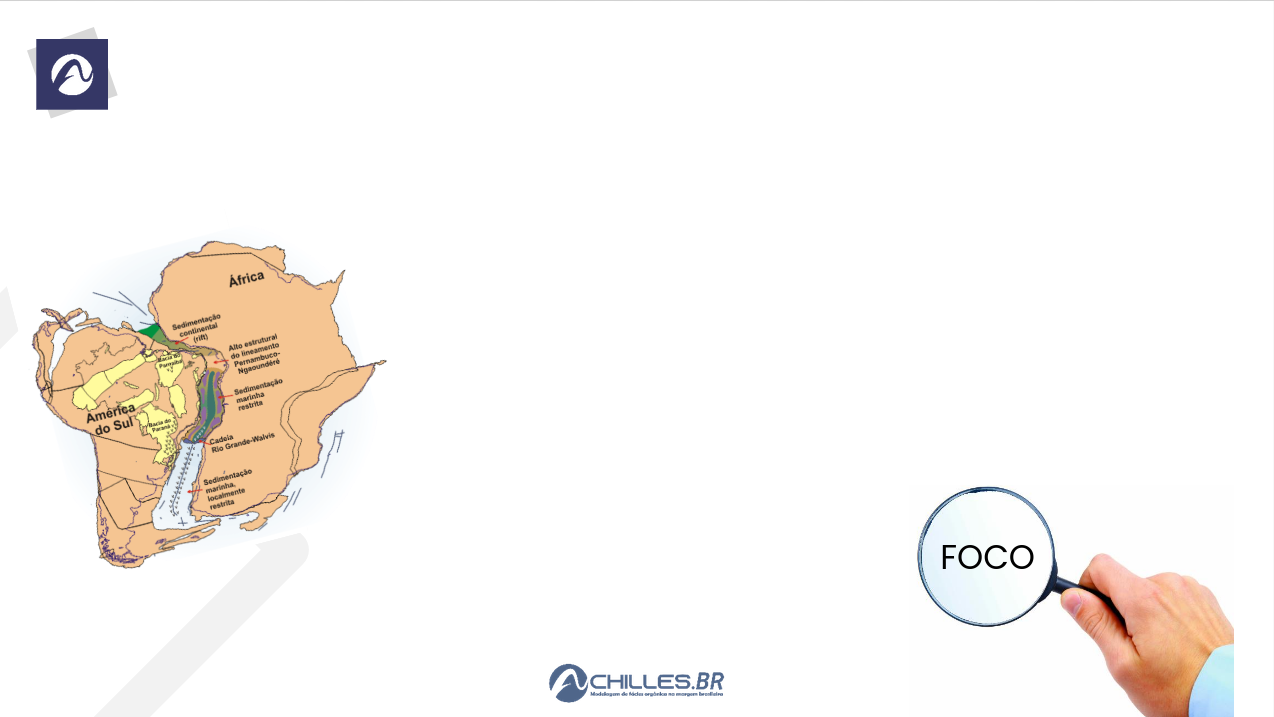
\includegraphics[width=\paperwidth,height=\paperheight]{images/sumario.png}
}

{ \begin{frame}
\begin{flushright}
\frametitle{Introdução}
\end{flushright}


\begin{flushright}
    \begin{columns}
    \column{0.4\textwidth}
        \centering
        
    \column{0.6\textwidth}
        \centering
	   Finalização do recebimento dos dados da ANP.
       Apresentar as amostras selecionadas, bem como as informações relacionadas aos custos de aquisição das mesmas.
	   Apresentar os avanços na ferramenta GeoPR4, Fuzzy Lakes, Odisséia.
	   Apresentar o aluno de IC.   
    \end{columns}

\end{flushright}


\end{frame} }





\section{Atualizações} % ATUALIZAR






\subsection{O modelo Fuzzy}

{
\usebackgroundtemplate{
\centering

\includegraphics[width=\paperwidth,height=\paperheight]{images/base.png}
}
\begin{frame}
\frametitle{Metodologia para cálculo do COT}
\begin{center}
	\smartdiagram[priority descriptive diagram]{Variáveis de entrada, Modelagem Fuzzy, Cálculo do erro}
\end{center}
\end{frame} 
}


{
\usebackgroundtemplate{
\centering

\includegraphics[width=\paperwidth,height=\paperheight]{images/base.png}
}
\begin{frame}
	\frametitle{Fuzzy Lakes}

\pause
	\begin{itemize}
		\item Objetivo: testar robustez do modelo frente à diminuição das variáveis de entrada
		\pause
		\item Recapitulando ... 
	\end{itemize}

\end{frame} 
}

{
\usebackgroundtemplate{
\centering

\includegraphics[width=\paperwidth,height=\paperheight]{images/base.png}
}
\begin{frame}

\frametitle{Recapitulando}
	\framesubtitle{Simulação: O Lago Victoria}
	\pause
	\begin{figure}
		\centering
		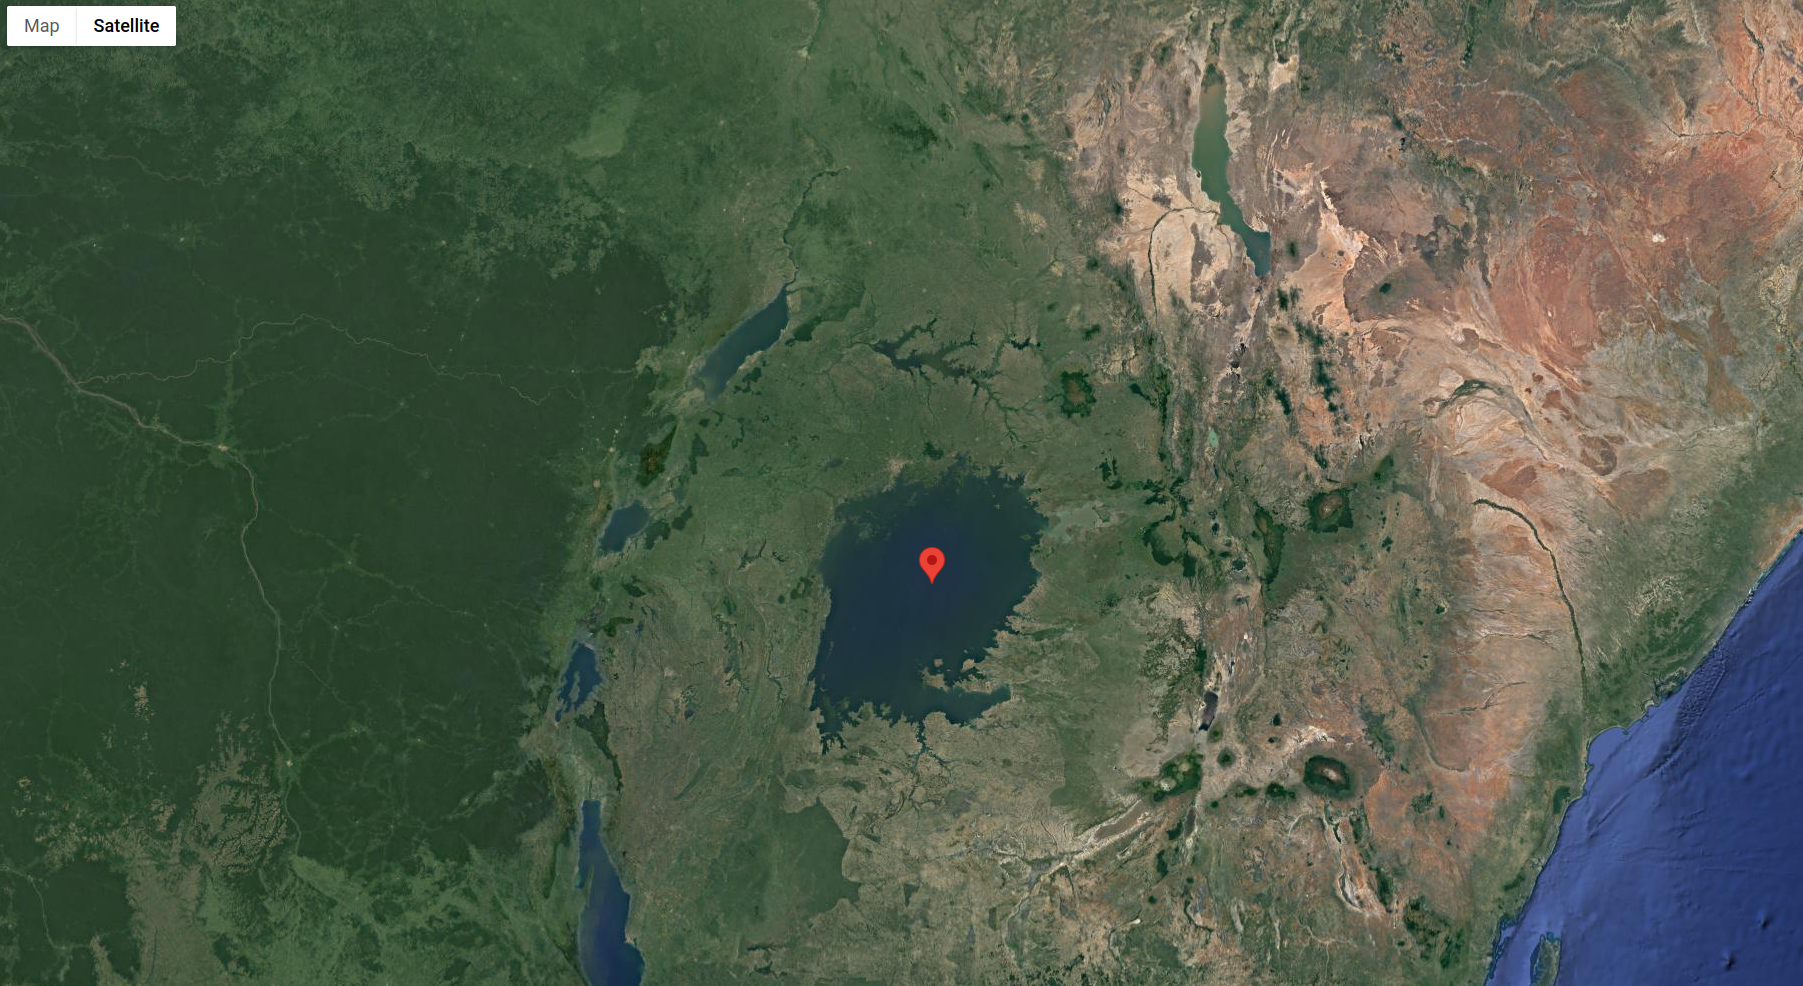
\includegraphics[scale=0.15]{images/victoria1.png}
	\end{figure}
\end{frame} 
}

{
\usebackgroundtemplate{
\centering

\includegraphics[width=\paperwidth,height=\paperheight]{images/base.png}
}
\begin{frame}

\frametitle{Recapitulando}
	\framesubtitle{Simulação: O Lago Victoria}
	\pause
	\begin{figure}
		\centering
		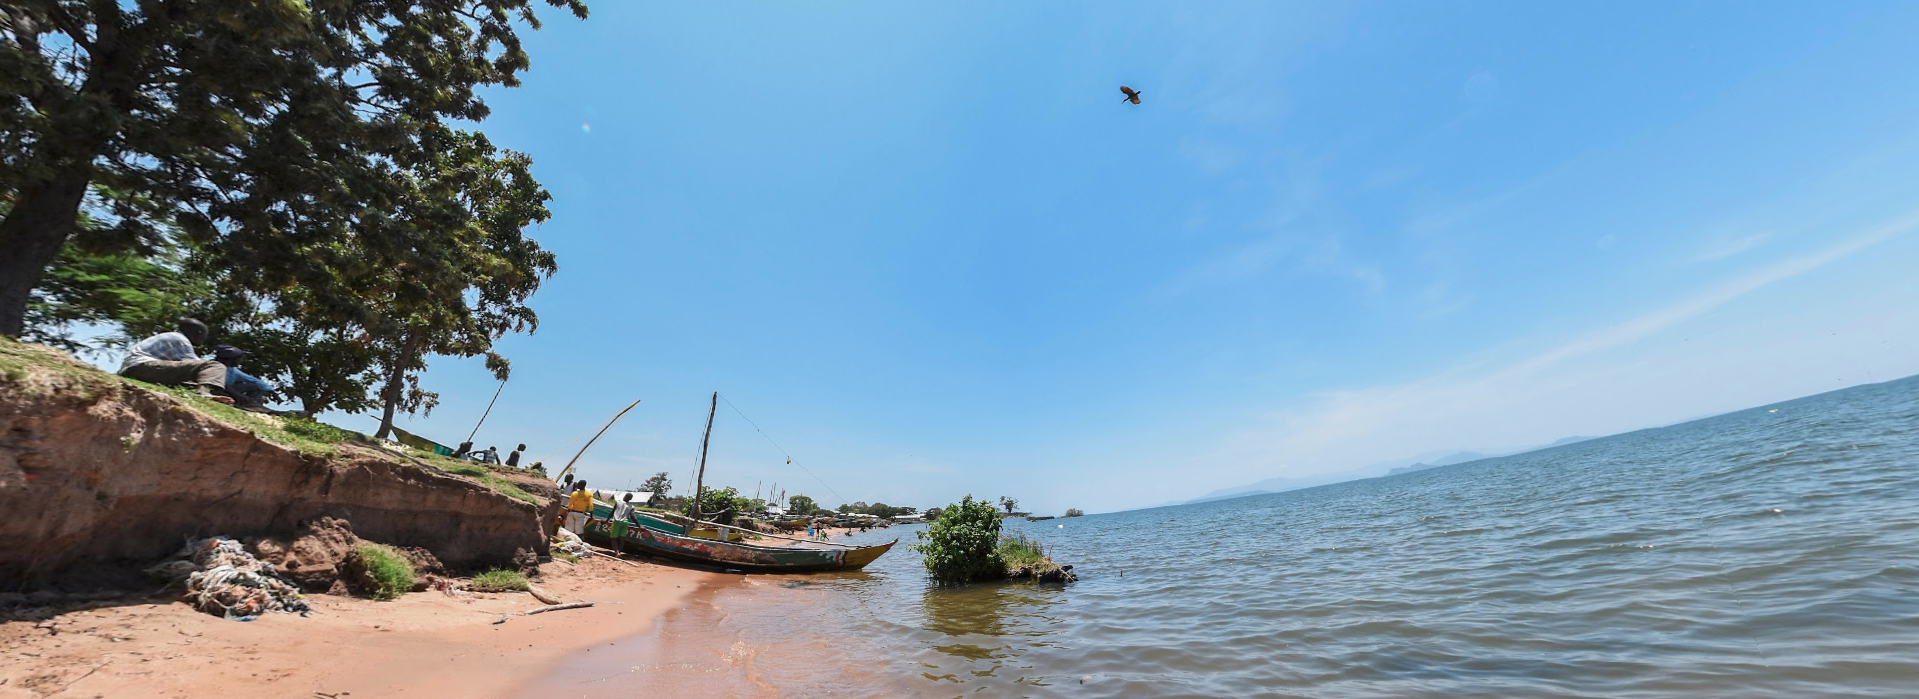
\includegraphics[scale=0.15]{images/victoria2.png}
	\end{figure}
\end{frame} 
}


{
\usebackgroundtemplate{
\centering

\includegraphics[width=\paperwidth,height=\paperheight]{images/base.png}
}
\begin{frame}

\frametitle{Recapitulando}
	\framesubtitle{Simulação: O Lago Victoria}
	\pause
	\begin{figure}
		\centering
		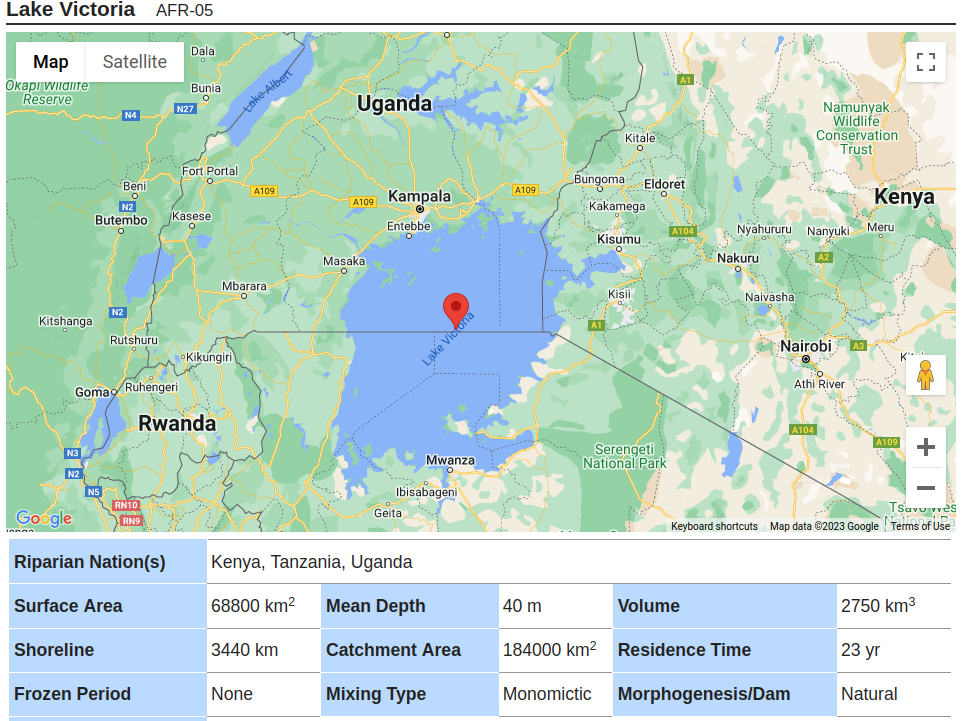
\includegraphics[scale=0.25]{images/victoria3.png}
	\end{figure}
\end{frame} 
}

{
\usebackgroundtemplate{
\centering

\includegraphics[width=\paperwidth,height=\paperheight]{images/base.png}
}
\begin{frame}

\frametitle{Recapitulando}
	\framesubtitle{Simulação: O Lago Tanganyika}
	\pause
	\begin{figure}
		\centering
		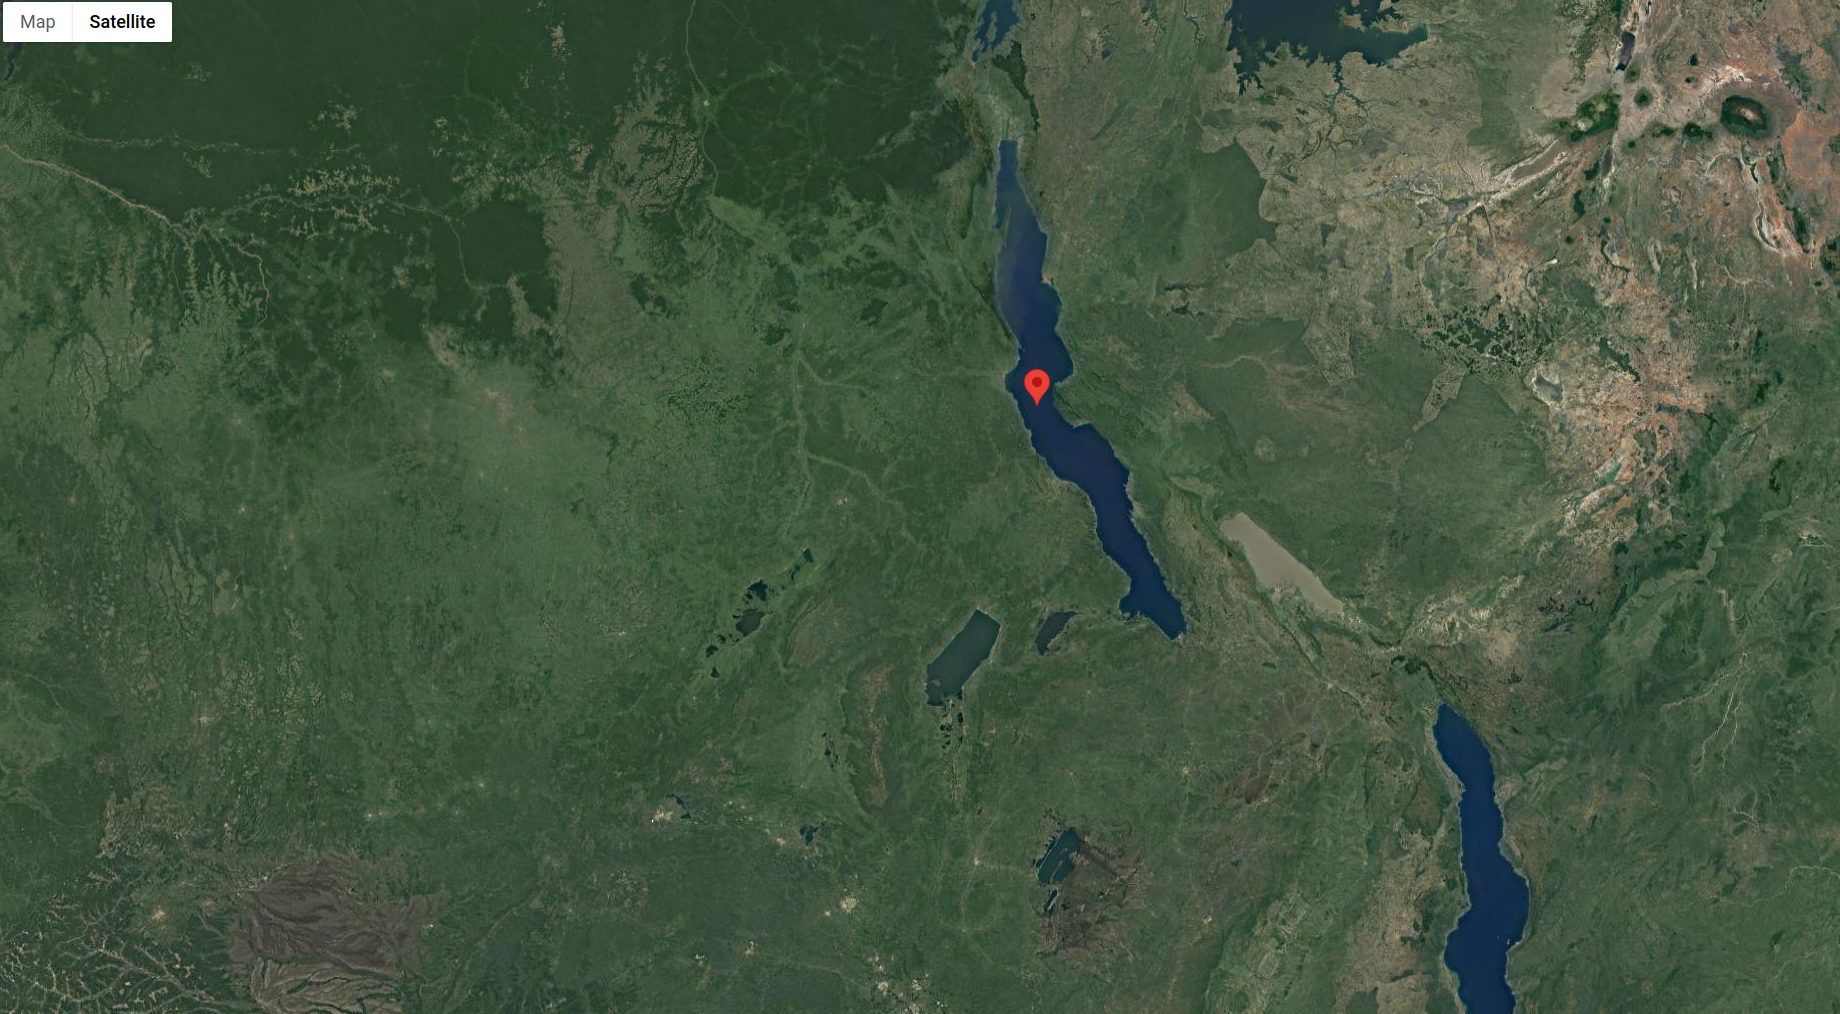
\includegraphics[scale=0.15]{images/Tanganyitka.png}
	\end{figure}
\end{frame} 
}

{
\usebackgroundtemplate{
\centering

\includegraphics[width=\paperwidth,height=\paperheight]{images/base.png}
}
\begin{frame}

\frametitle{Recapitulando}
	\framesubtitle{Simulação: O Lago Tanganyika}
	\pause
	\begin{figure}
		\centering
		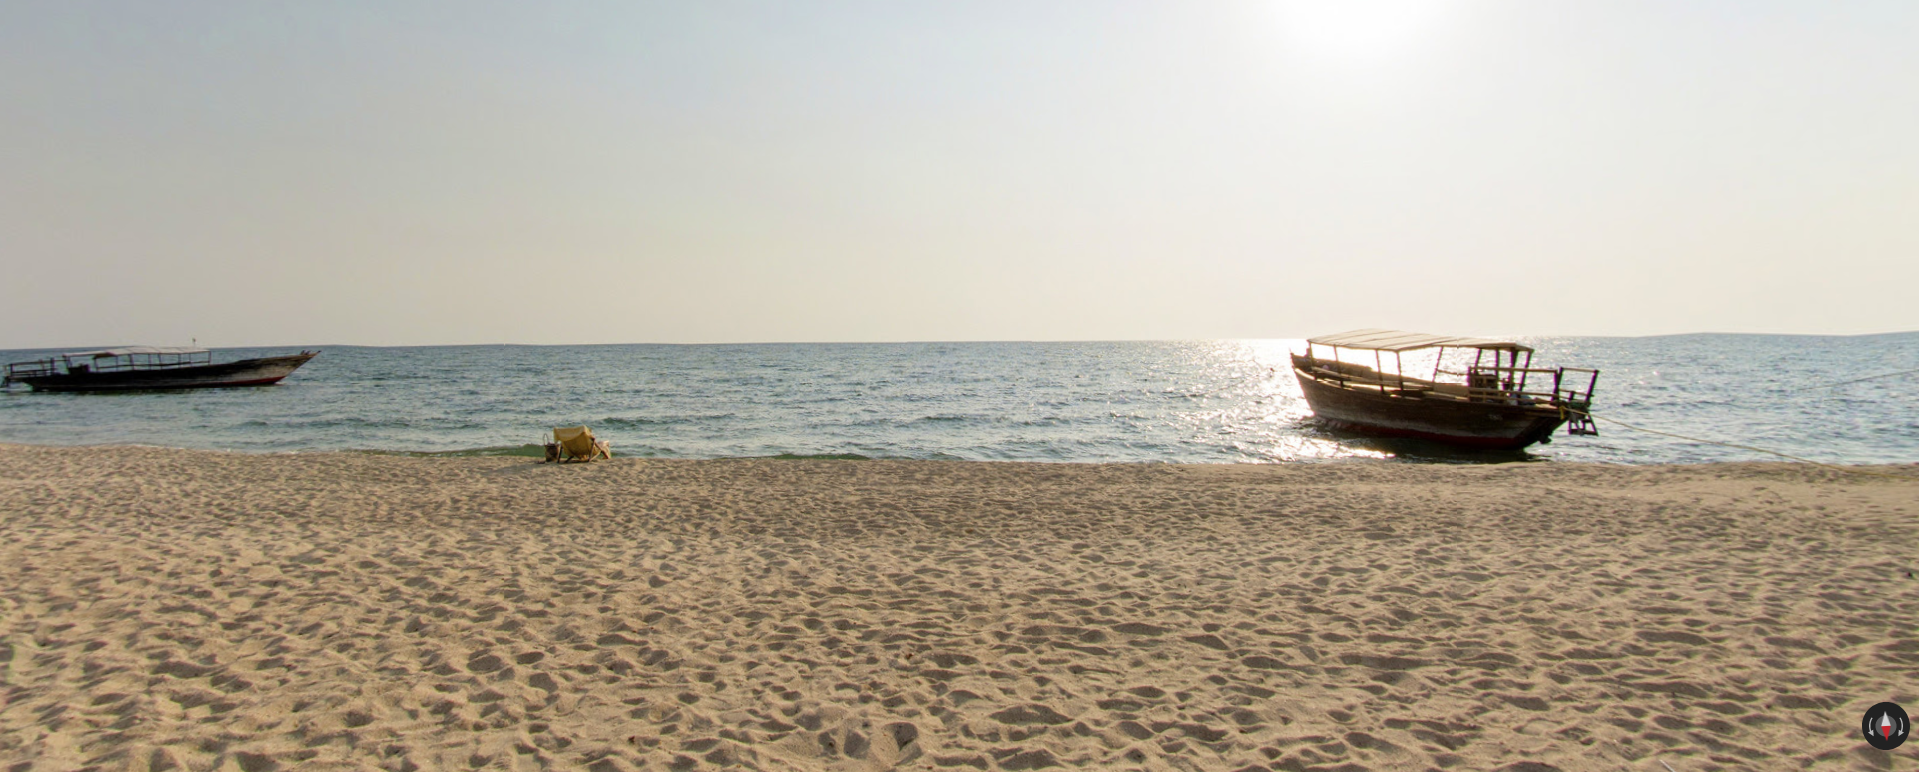
\includegraphics[scale=0.15]{images/Tanganyika2.png}
	\end{figure}
\end{frame} 
}

{
\usebackgroundtemplate{
\centering

\includegraphics[width=\paperwidth,height=\paperheight]{images/base.png}
}
\begin{frame}

\frametitle{Recapitulando}
	\framesubtitle{Simulação: O Lago Tanganyika}
	\pause
	\begin{figure}
		\centering
		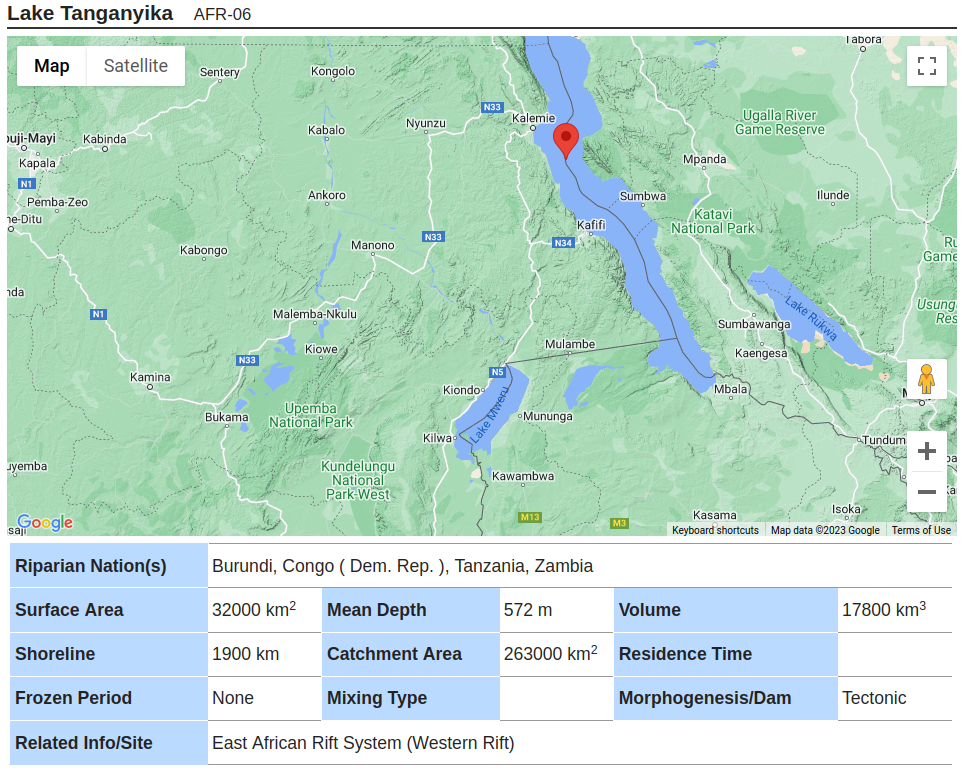
\includegraphics[scale=0.25]{images/Tanganyika3.png}
	\end{figure}
\end{frame} 
}

{
\usebackgroundtemplate{
\centering

\includegraphics[width=\paperwidth,height=\paperheight]{images/base.png}
}
\begin{frame}

\frametitle{Recapitulando}
	\framesubtitle{Simulação: O Lago Kivu}
	\pause
	\begin{figure}
		\centering
		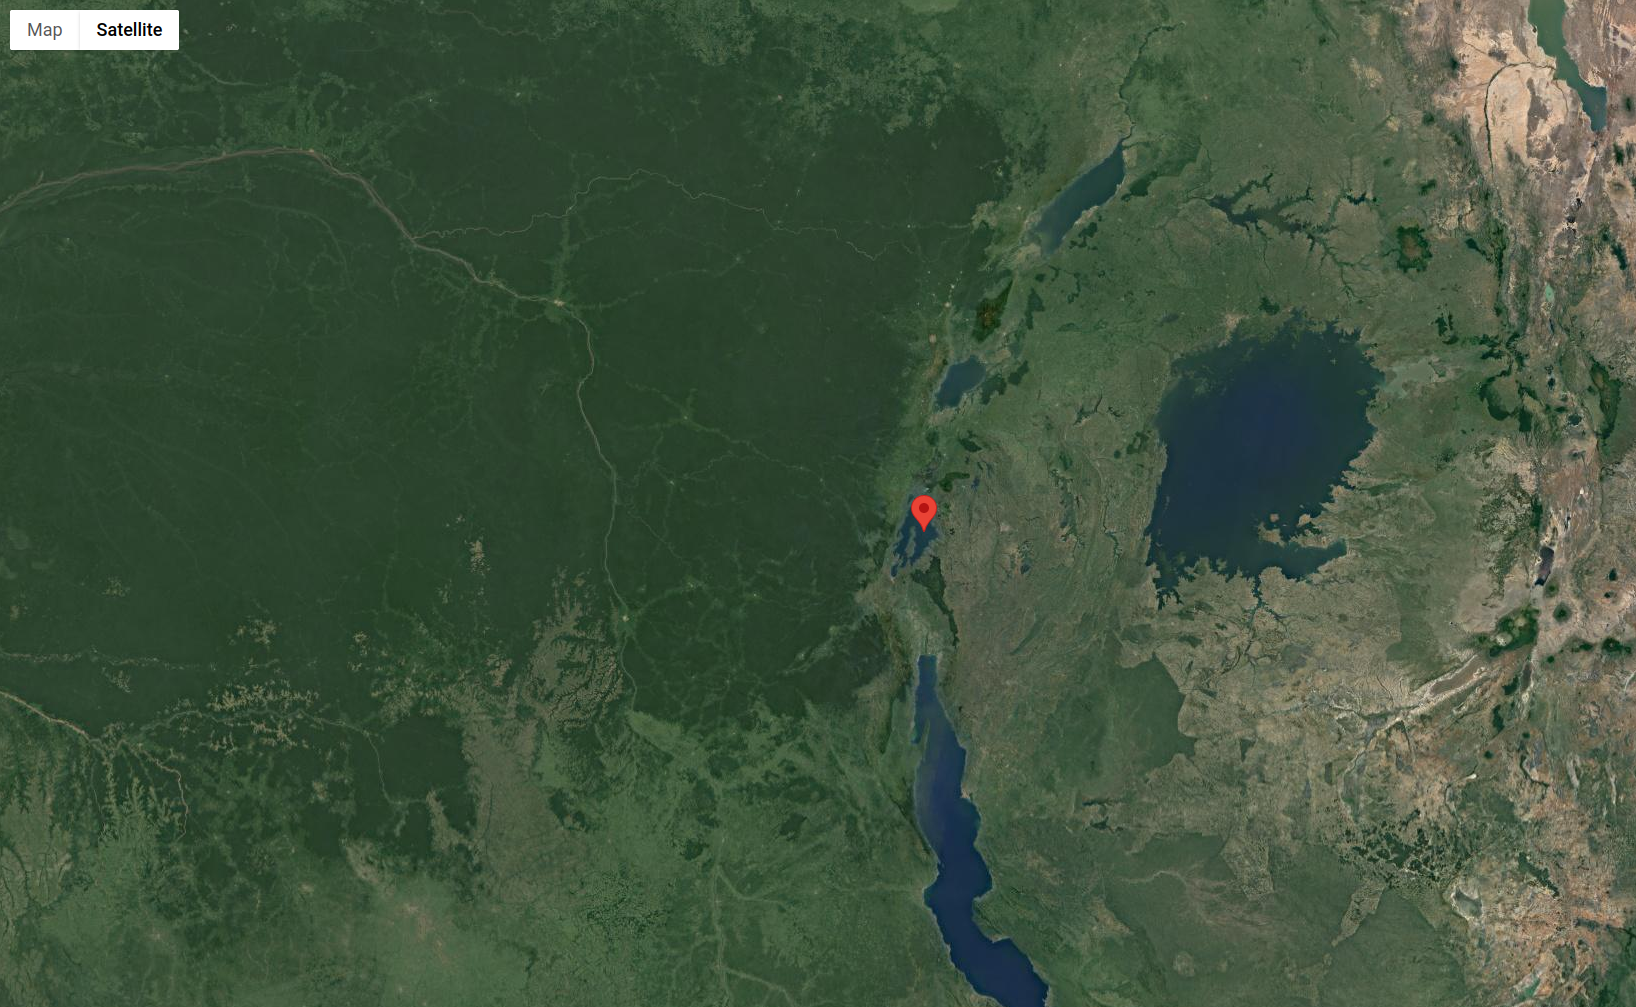
\includegraphics[scale=0.15]{images/kivu1.png}
	\end{figure}
\end{frame} 
}


{
\usebackgroundtemplate{
\centering

\includegraphics[width=\paperwidth,height=\paperheight]{images/base.png}
}
\begin{frame}

\frametitle{Recapitulando}
	\framesubtitle{Simulação: O Lago Kivu}
	\pause
	\begin{figure}
		\centering
		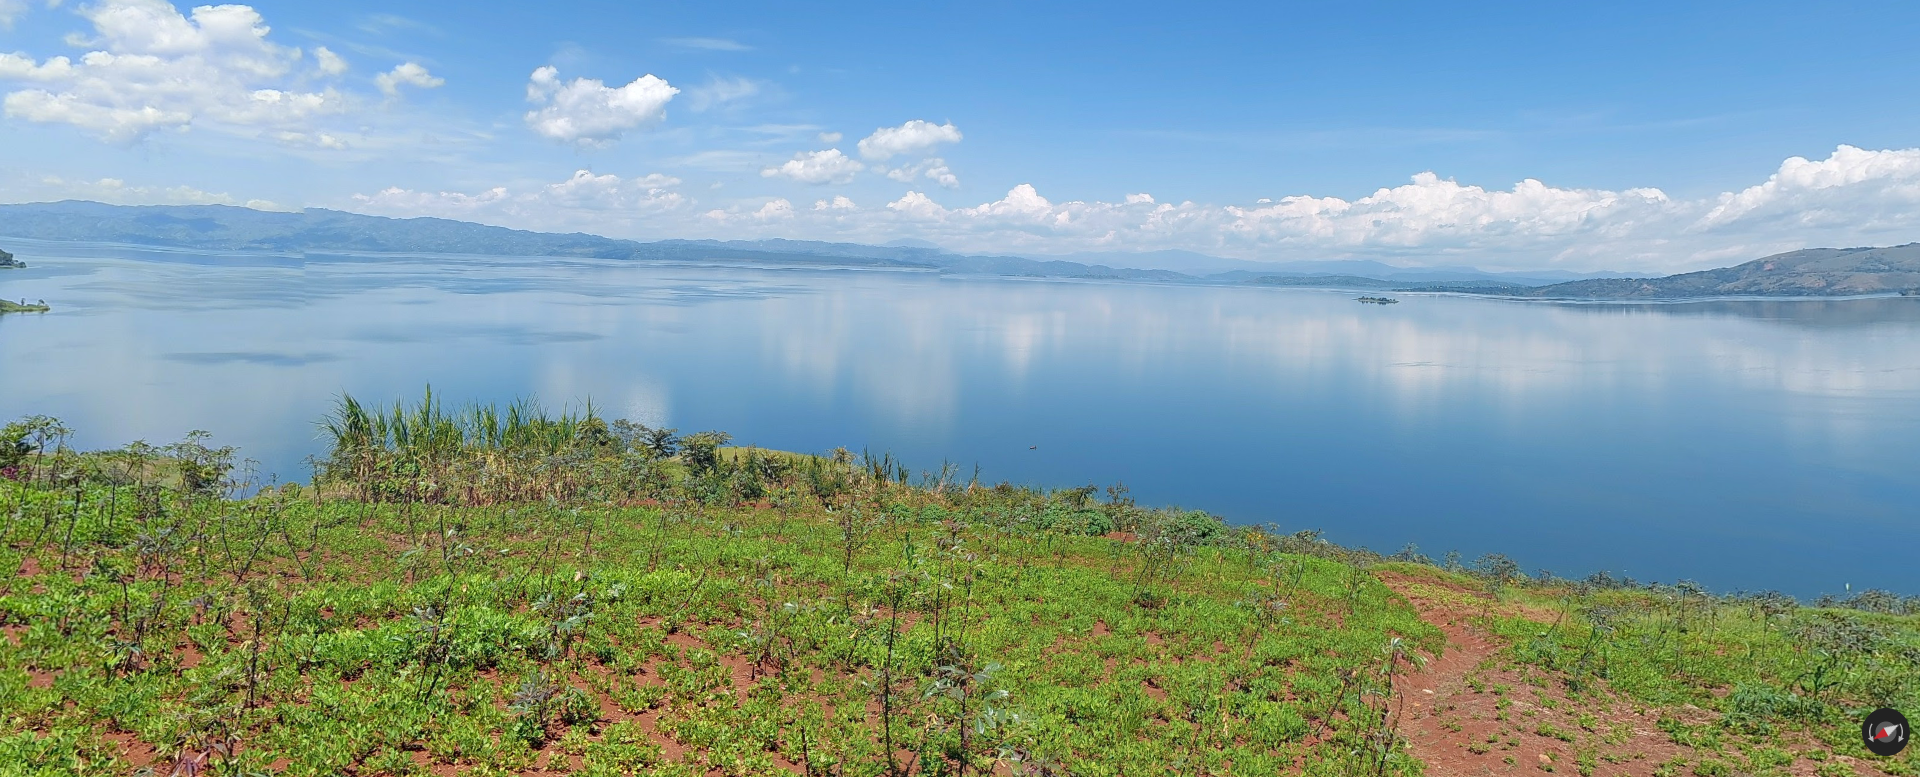
\includegraphics[scale=0.15]{images/kivu2.png}
	\end{figure}
\end{frame} 
}




{
\usebackgroundtemplate{
\centering

\includegraphics[width=\paperwidth,height=\paperheight]{images/base.png}
}
\begin{frame}

\frametitle{Recapitulando}
	\framesubtitle{Simulação: O Lago Kivu}
	\pause
	\begin{figure}
		\centering
		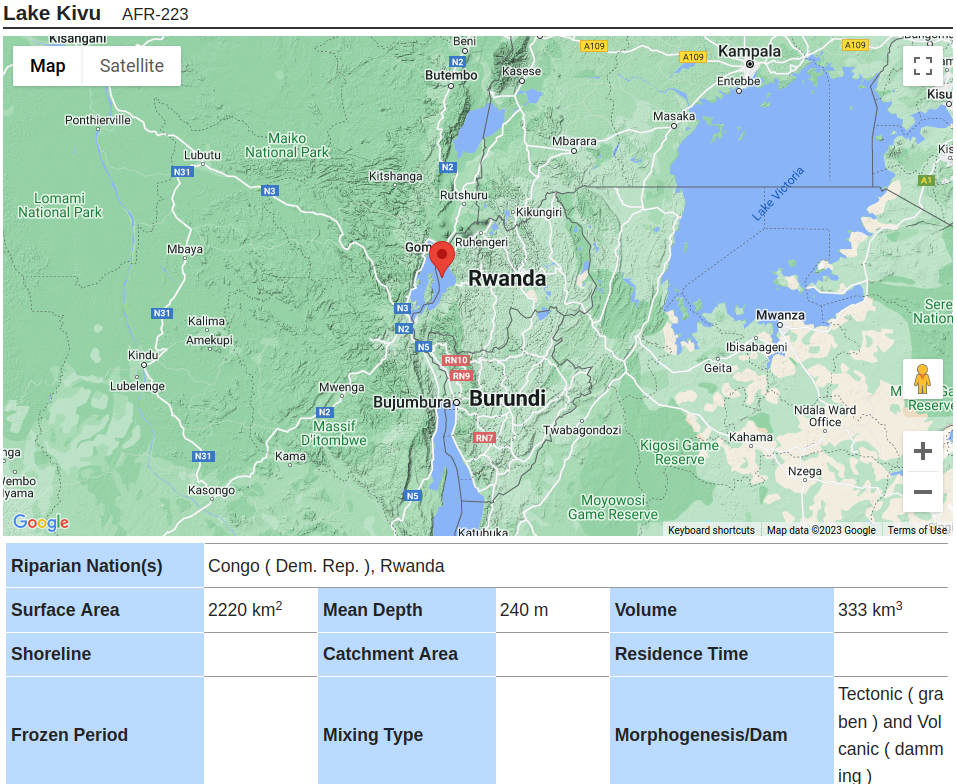
\includegraphics[scale=0.25]{images/kivu3.png}
	\end{figure}
\end{frame} 
}


{
\usebackgroundtemplate{
\centering

\includegraphics[width=\paperwidth,height=\paperheight]{images/base.png}
}
\begin{frame}
\frametitle{O modelo fuzzy - V.01} 
\begin{figure}
\centering
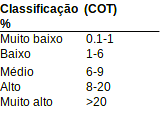
\includegraphics[scale=0.2]{tabela_fuzzy.png}
\end{figure}
\pause
	\begin{itemize}
		\item Modelo possui 6 variáveis antecedentes e 1 conseqüente
		\pause
		\item Função de pertinência triangular
		\pause
		\item 18 Regras
	\end{itemize}
\end{frame} 
}


{
\usebackgroundtemplate{
\centering

\includegraphics[width=\paperwidth,height=\paperheight]{images/base.png}
}
\begin{frame}
\frametitle{Teste do número de variáveis de entrada (RN1)} 
\begin{figure}
\centering
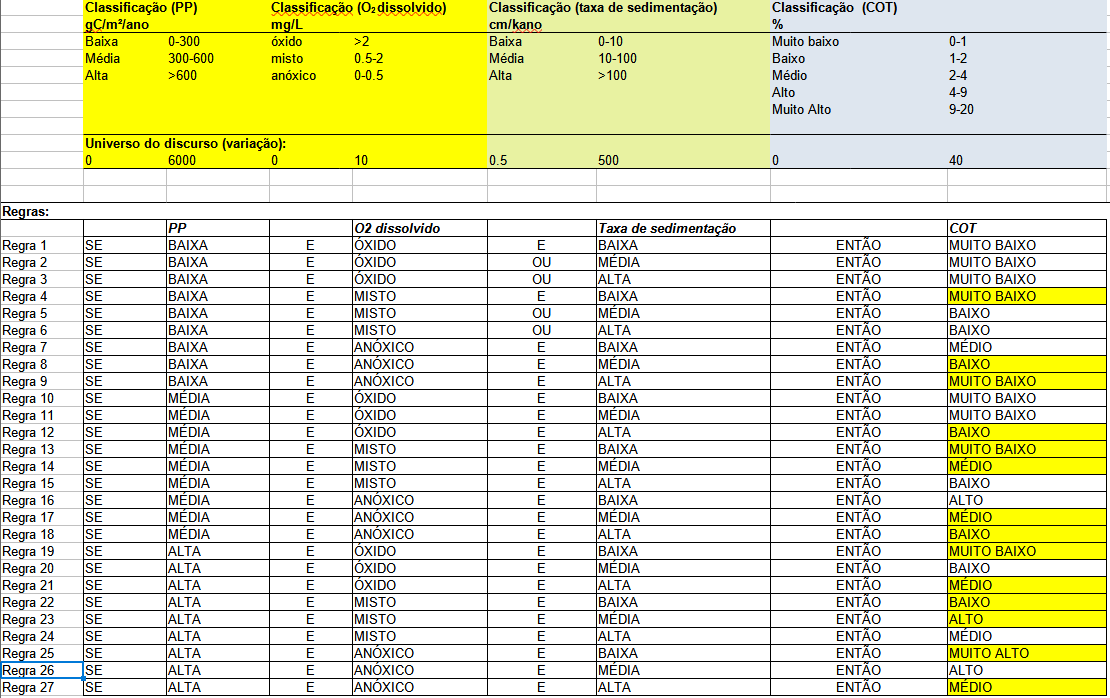
\includegraphics[scale=0.2]{FuzzyRN1.png}
\end{figure}
\pause
	\begin{itemize}
		\item Modelo possui 3 variáveis antecedentes e 1 conseqüente
		\pause
		\item Função de pertinência triangular
		\pause
		\item 27 Regras
	\end{itemize}
\end{frame} 
}


{
\usebackgroundtemplate{
\centering

\includegraphics[width=\paperwidth,height=\paperheight]{images/base.png}
}
\begin{frame}
\frametitle{Teste do número de variáveis de entrada (RN2)} 
\begin{figure}
\centering
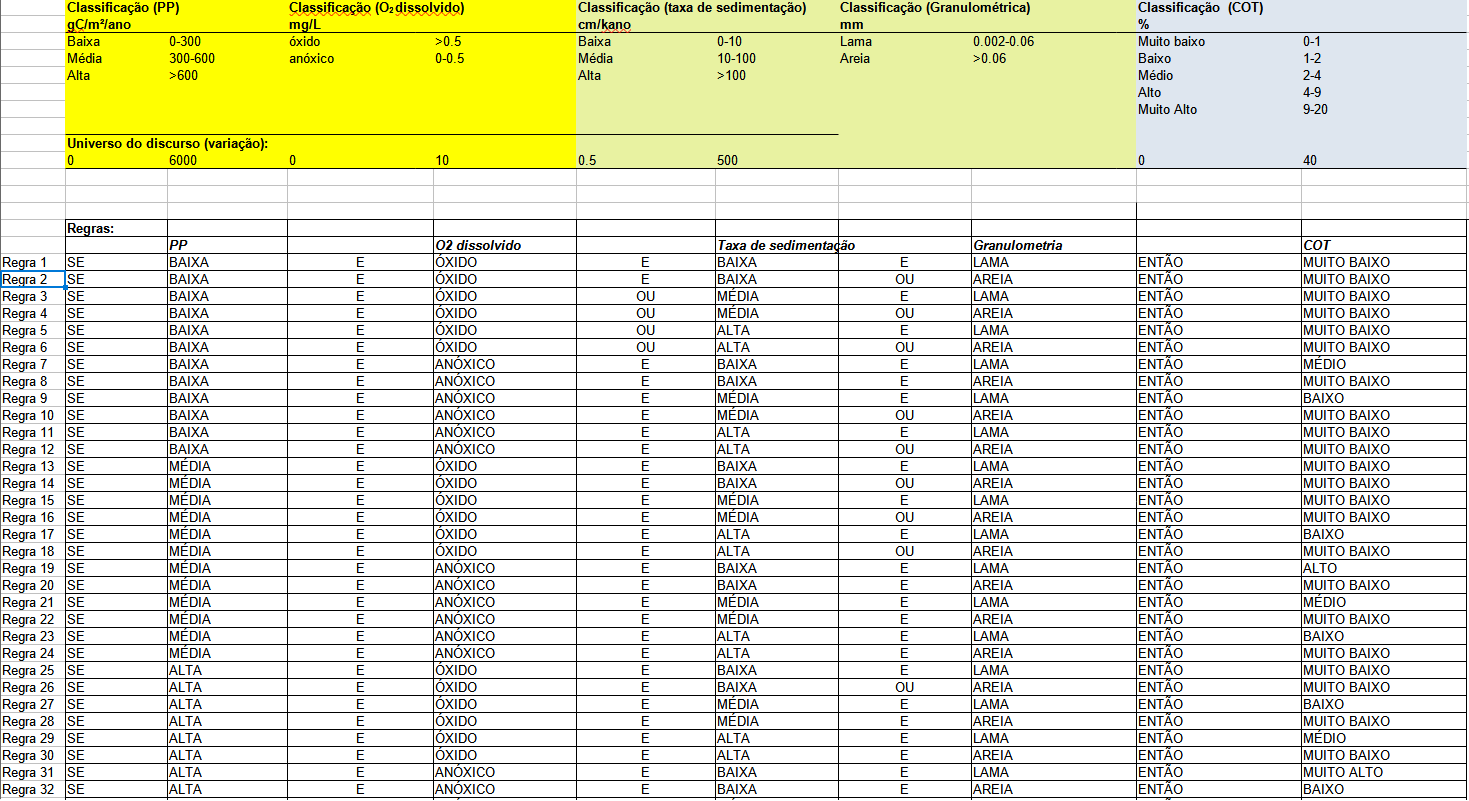
\includegraphics[scale=0.2]{FuzzyRN2.png}
\end{figure}
\pause
	\begin{itemize}
		\item Modelo possui 4 variáveis antecedentes e 1 conseqüente
		\pause
		\item Função de pertinência triangular
		\pause
		\item 36 Regras
	\end{itemize}
\end{frame} 
}



{
\usebackgroundtemplate{
\centering

\includegraphics[width=\paperwidth,height=\paperheight]{images/base.png}
}
\begin{frame}
\frametitle{Tabela dos dados de entrada da modelagem Fuzzy}
\begin{figure}
\centering
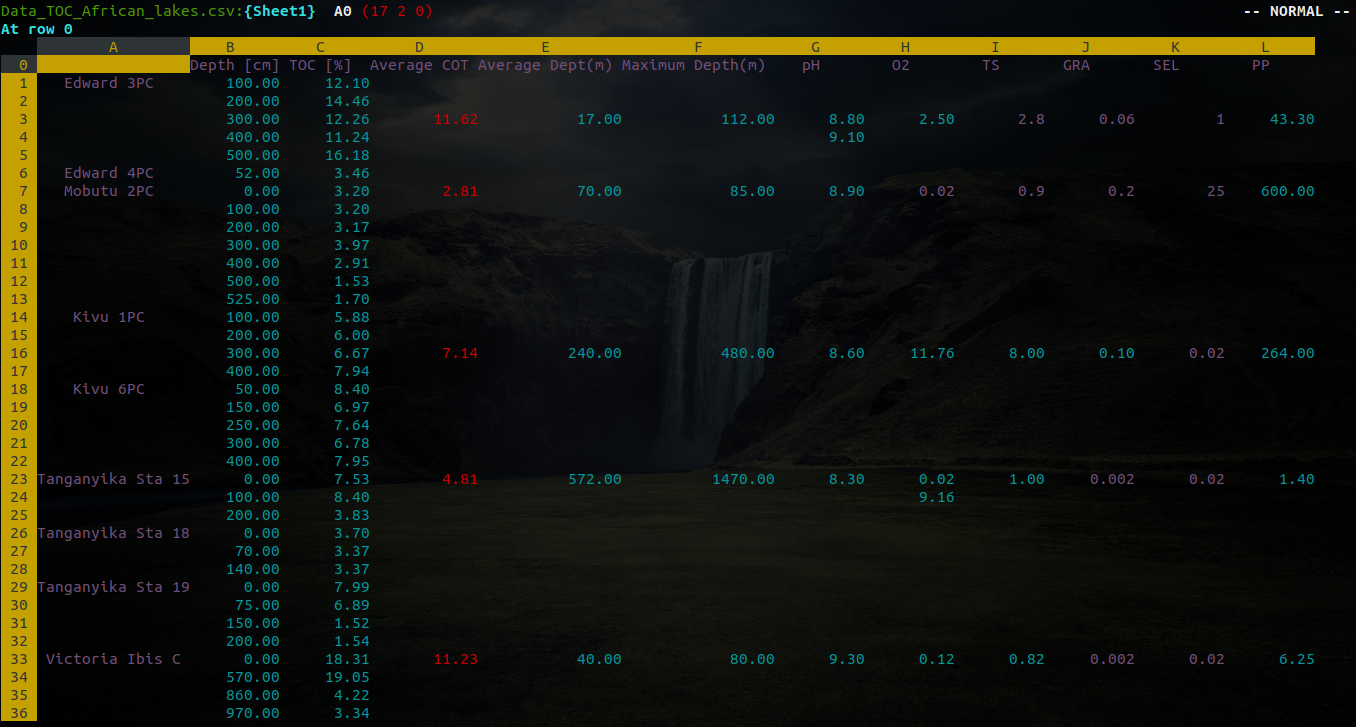
\includegraphics[scale=0.25]{entradas_fuzzy.png}
\end{figure}
\end{frame} 
}

{
\usebackgroundtemplate{
\centering

\includegraphics[width=\paperwidth,height=\paperheight]{images/base.png}
}
\begin{frame}
\frametitle{Resultados}
\begin{table}[htbp]
	\centering
	\caption{Resultado do teste (Erro \%)}
	\label{tab:variaveis}
	\begin{tabular}{c|c|c|c|}
	\hline
	& L. Kivu & L. Tanganyika & L. Victoria \\
	\hline
	Modelo Fuzzy v01& 0.53 & 0.13 & 0.35 \\
	Modelo teste RN1& 6.42 & 9.96 & 7.65 \\
	Modelo teste RN2& 6.54 & 4.12 & 6.85 \\
	% Add more rows as needed
	\hline
	\end{tabular}
	\end{table}
	
\end{frame} 
}


\subsection{GeoPR4, Seleção de amostras}

{
\usebackgroundtemplate{
\centering

\includegraphics[width=\paperwidth,height=\paperheight]{images/base.png}
}
\begin{frame}
	\frametitle{GeoPR4 - localização das geradoras}

	    \begin{figure}
		    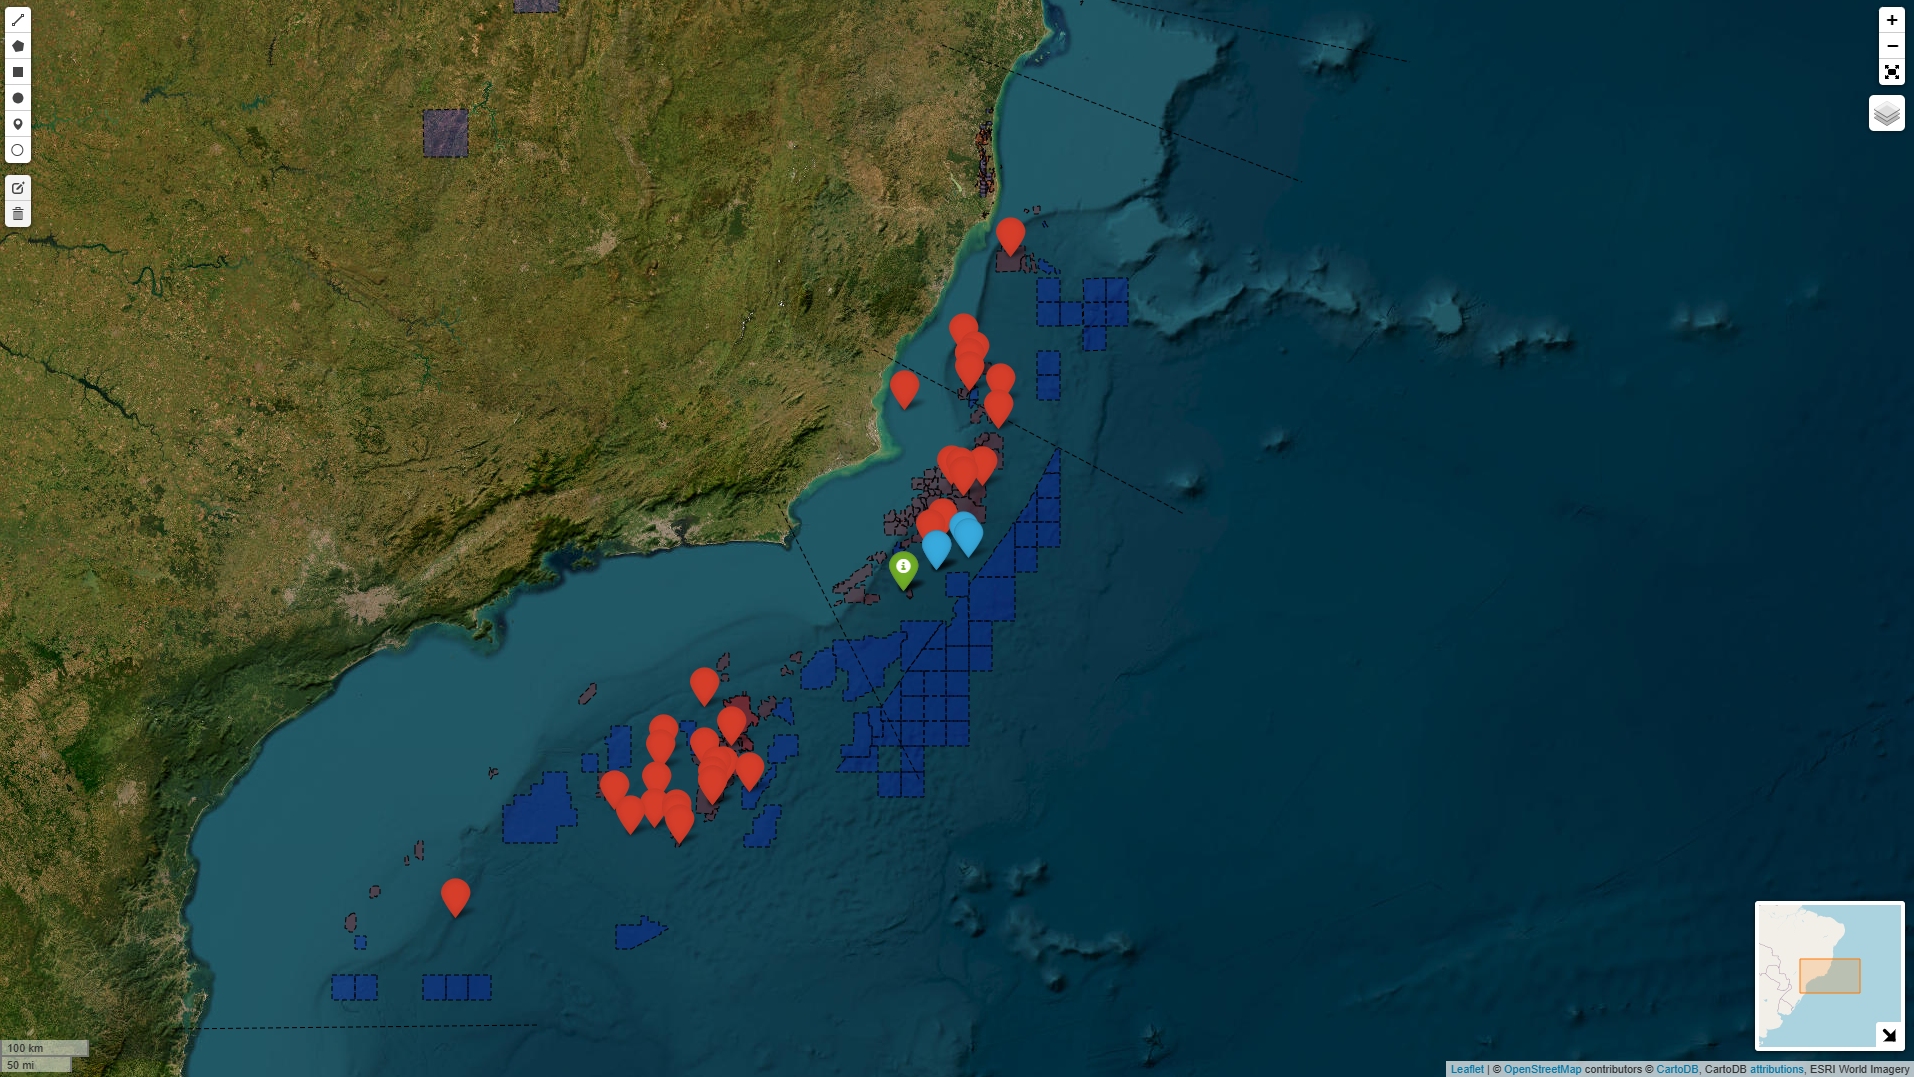
\includegraphics[scale=0.2]{images/GeoPR4_loc.png}
	    \end{figure}
	\begin{itemize}
		\item Aproximadamente 35 poços
                \pause
		\item Bacias = Campos, Espírito Santo, Santos 
	\end{itemize}
\end{frame} 
}


{
\usebackgroundtemplate{
\centering

\includegraphics[width=\paperwidth,height=\paperheight]{images/base.png}
}
\begin{frame}
	\frametitle{Horizontes das escolha amostrais}
   \begin{center}
		Existem 10 poços não possuem dados de geoquímica, nas Bacias de Campos e de Santos 
   \end{center}

	\begin{center}
		\smartdiagram[priority descriptive diagram]{Tratamento de dados, 
		 localização da geradora, estimativa do COT, seleção amostral}
	\end{center}


\end{frame} 
}


{
\usebackgroundtemplate{
\centering

\includegraphics[width=\paperwidth,height=\paperheight]{images/base.png}
}
\begin{frame}
	\frametitle{Horizontes das escolhas amostrais}

	\begin{figure}
		\flushright
		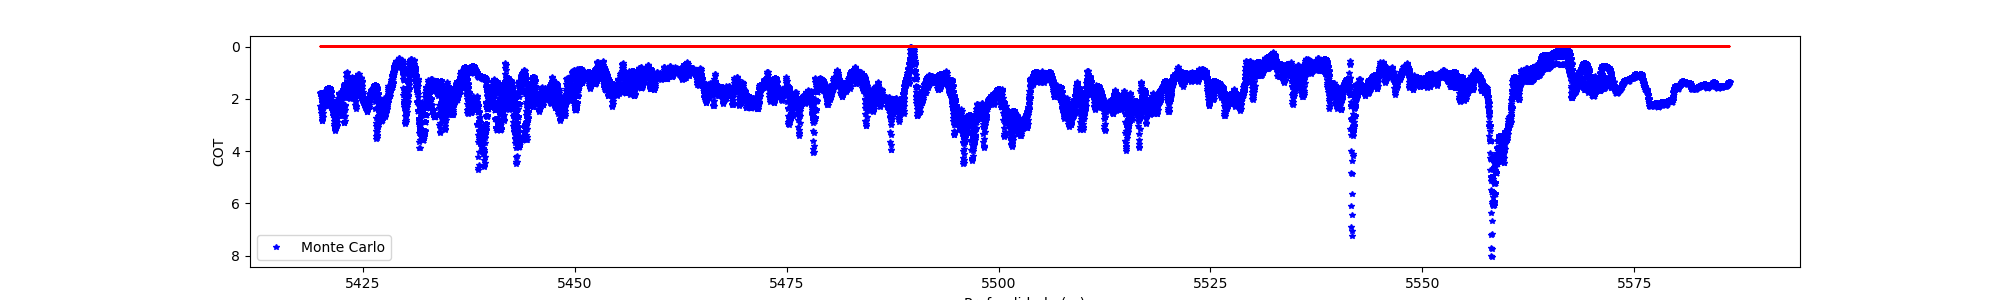
\includegraphics[scale=0.25]{images/1BRSA1007RJS.png}
	\end{figure}
	
		\begin{columns}[c] % centralizar verticalmente as colunas
			\column{.5\textwidth} % largura da primeira coluna (50% do espaço disponível)
			\centering
			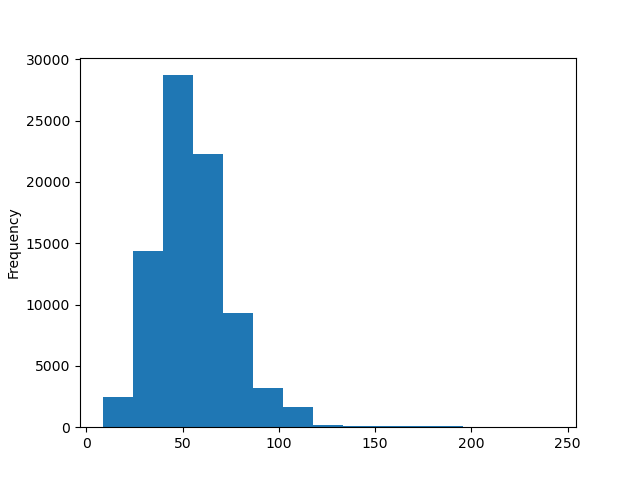
\includegraphics[scale=0.3]{images/GR_1BRSA1007RJS.png} % substitua "figura1" pelo nome do arquivo da primeira imagem
		
			\column{.5\textwidth} % largura da segunda coluna (50% do espaço disponível)
			\centering
			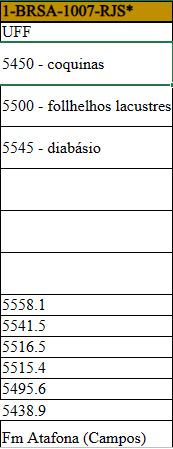
\includegraphics[scale=0.4]{images/amostragem1BRSA1007RJS.png} % substitua "figura2" pelo nome do arquivo da segunda imagem
		  \end{columns}
    Total: 35 amostras para Bacia de Santos e 24 amostras para Bacia de Campos. 

\end{frame} 
}


{
\usebackgroundtemplate{
\centering

\includegraphics[width=\paperwidth,height=\paperheight]{images/base.png}
}
\begin{frame}
	\frametitle{Informações importantes}

	\begin{itemize}
		\item Não existe um limite para solicitação de amostras, o que existe é um limite anual para solicitação de poços (20 por ano). Além disso, pode acontecer de não ser possível disponibilizar o quantitativo total requerido de amostras de calha caso a empresa depositária das amostras informe que a quantia em questão faz parte do mínimo de preservação, conforme exigência da resolução ANP nº 71/2014. Entretanto, em regra não existe limite para solicitação de amostras.
		\pause
		\item Existe a possibilidade de solicitar tanto lâminas prontas (pré-existentes) quanto amostras para confecção de lâminas, se for preciso.
        \pause
		\item O valor final em reais é dado pela depositária nas etapas subsequentes à formalização da solicitação de acesso a amostras. Os valores praticados pela Equinor, em 2022, para calha são R\$ $72,21$ por caixa, R\$ $182,49$ para amostra lateral e R\$ $677,16$ o metro 
	\end{itemize}
\end{frame} 
}



\subsection{Dados ANP}

{
\usebackgroundtemplate{
\centering

\includegraphics[width=\paperwidth,height=\paperheight]{images/base.png}
}
\begin{frame}
	\frametitle{Atualização da requisição de dados}

	    \begin{figure}
		    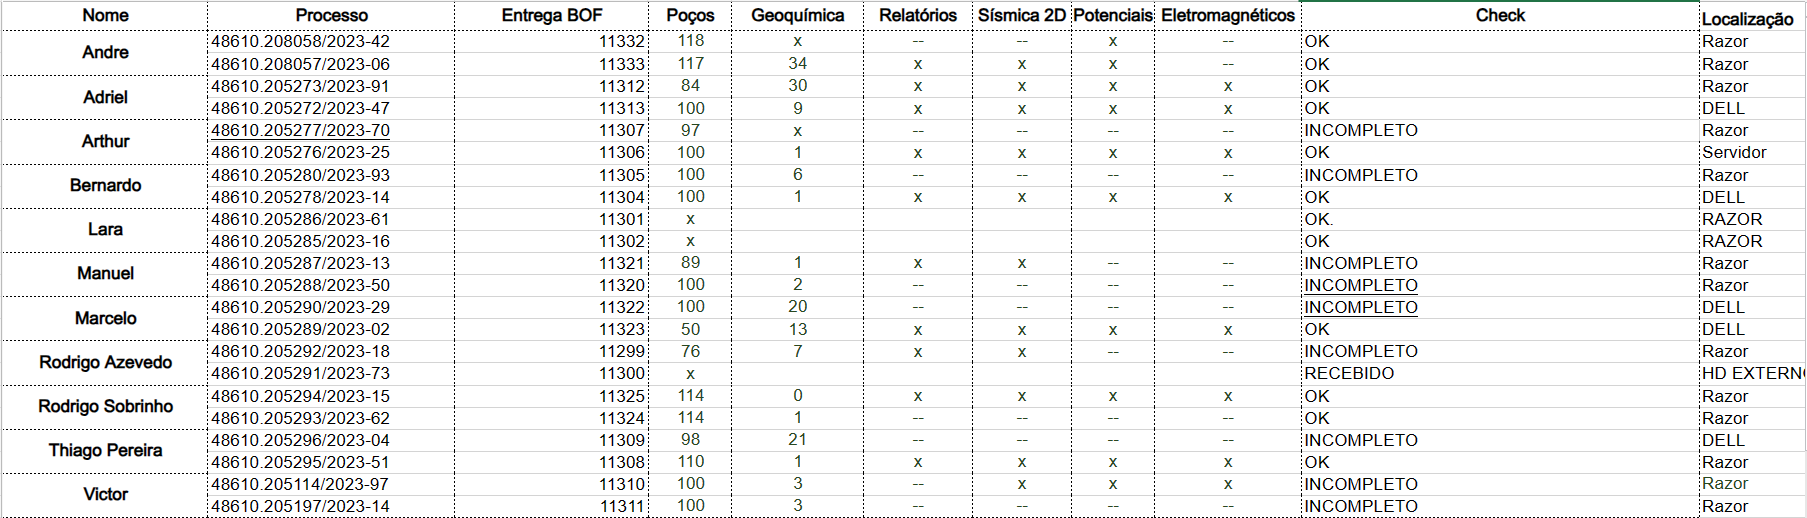
\includegraphics[scale=0.2]{images/ANPdados.png}
	    \end{figure}
	\begin{itemize}
		\item Aproximadamente dados de 1900 poços
                \pause
		\item Bacias = Alagoas, Acre,  Amazonas, Foz do Amazonas, Campos, Ceará, Espírito Santo, Santos, Tucano (Norte, Central, Sul), Jatobá 
	\end{itemize}
\end{frame} 
}

\subsection{Banco de dados }

{
\usebackgroundtemplate{
\centering

\includegraphics[width=\paperwidth,height=\paperheight]{images/base.png}
}
\begin{frame}
	\frametitle{Banco de dados}



	    \begin{figure}
		    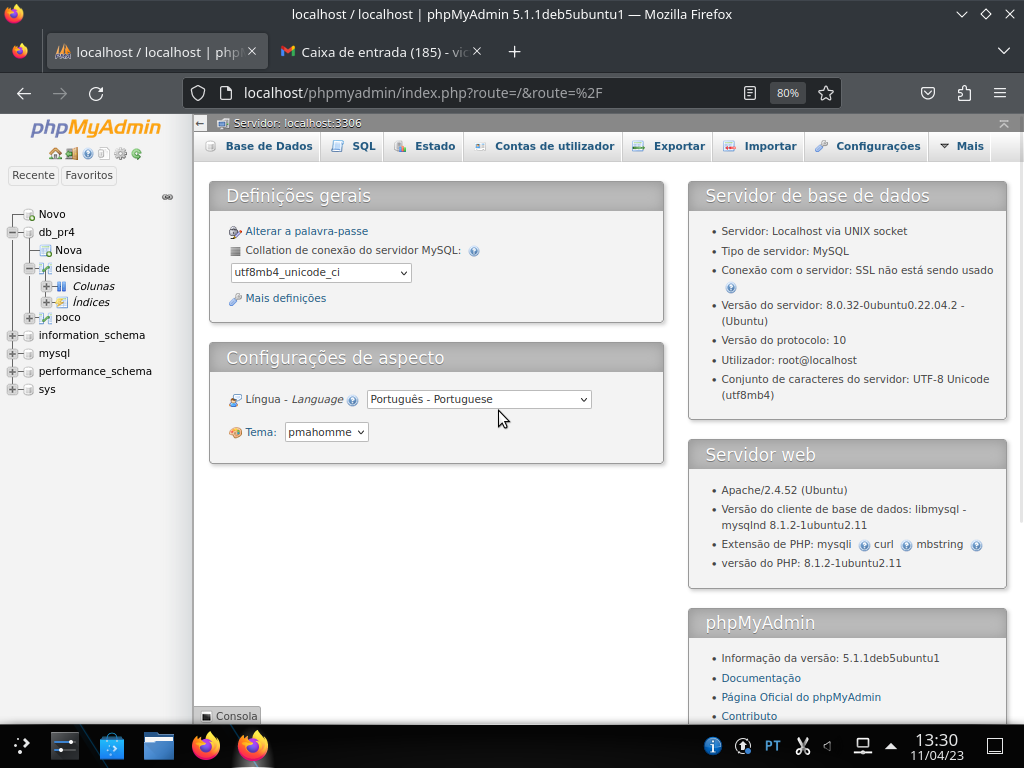
\includegraphics[scale=0.3]{images/BD.png}
	    \end{figure}

\pause
	\begin{itemize}
		\item necessário modificar o cabeçalho dos dados para que a busca SQL funcione (Em desenvolvimento)
	\end{itemize}

\end{frame} 
}


\subsection{Seleção bolsista de IC}


{
\usebackgroundtemplate{
\centering

\includegraphics[width=\paperwidth,height=\paperheight]{images/base.png}
}
\begin{frame}
	\frametitle{Seleção IC}



	    \begin{figure}
		    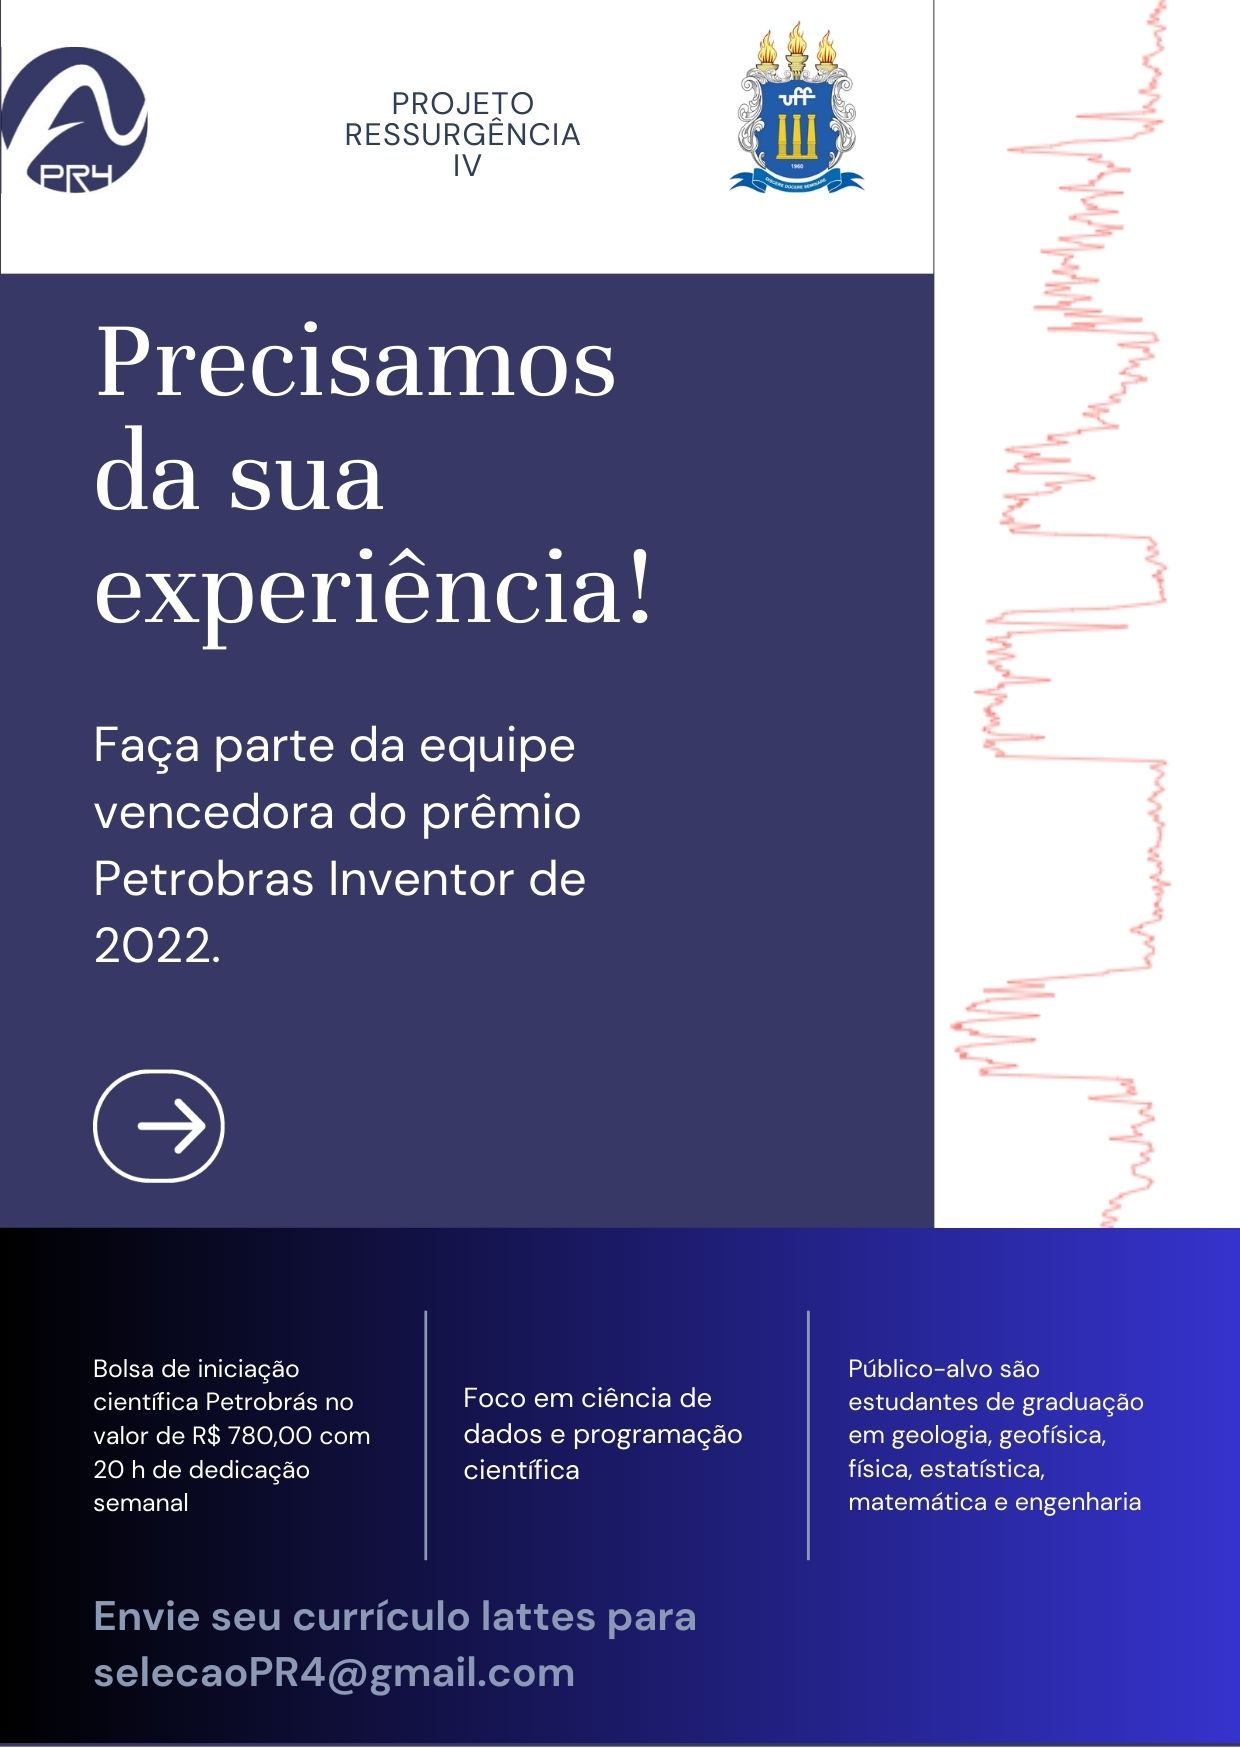
\includegraphics[scale=0.4]{images/Bolsa_IC1.jpg}
	    \end{figure}

\end{frame} 
}

{
\usebackgroundtemplate{
\centering

\includegraphics[width=\paperwidth,height=\paperheight]{images/base.png}
}
\begin{frame}
	\frametitle{Seleção IC}



	    \begin{figure}
		    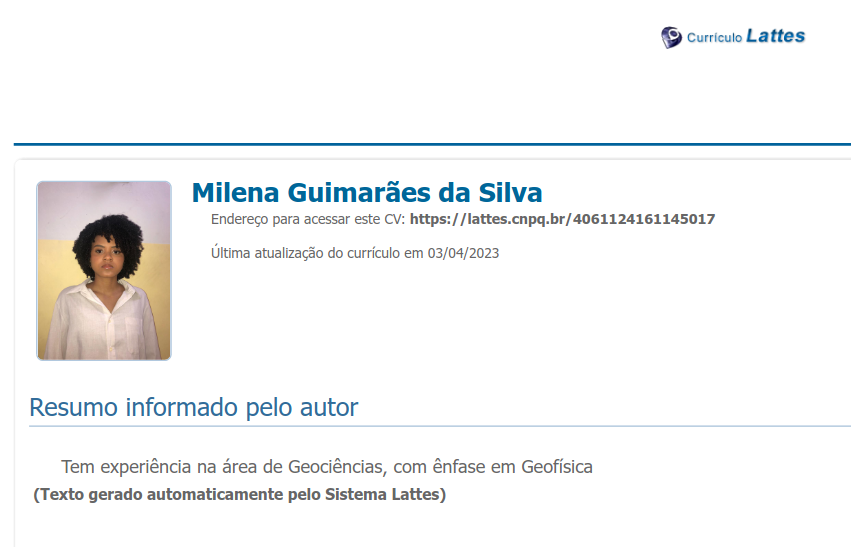
\includegraphics[scale=0.3]{images/AlunaIC.png}
	    \end{figure}
              Início em 01 de Junho de 2023. 
\end{frame} 
}






{
\usebackgroundtemplate{
\centering

\includegraphics[width=\paperwidth,height=\paperheight]{images/base.png}
}
\begin{frame}[allowframebreaks]
\frametitle{Referências}
%\beamertemplatetextbibitems
\tiny
\bibliographystyle{apalike}
\bibliography{references}
\end{frame}
}
\makeatother

{
\usebackgroundtemplate{
\centering

\includegraphics[width=\paperwidth,height=\paperheight]{images/interlocucao.png}
}
	
% Frame 3: plano de fundo
\begin{frame}

	
\end{frame}
}

{
\usebackgroundtemplate{
\centering
\includegraphics[width=\paperwidth,height=\paperheight]{images/agradecimento.png}
}
	
% Frame 3: plano de fundo
\begin{frame}
	
\end{frame}
}
\end{document}
